% Figure for scale_lanes deck: The agentic-RL loop: AgentCore is the sandbox tier.
% Build: xelatex lanes_fig02_rl-loop.tex  (-> .pdf, included by ../aws/scale_lanes.tex)
\documentclass[tikz,border=4pt]{standalone}
\usepackage{fontspec}
\setmainfont{DejaVu Sans}
\setmonofont{DejaVu Sans Mono}
\usetikzlibrary{positioning,arrows.meta,fit,backgrounds,calc,decorations.pathreplacing}
\definecolor{slime}{RGB}{230,230,230}
\definecolor{host}{RGB}{214,216,240}
\definecolor{gpu}{RGB}{255,236,204}
\definecolor{vm}{RGB}{214,238,220}
\definecolor{ac}{RGB}{255,246,230}
\definecolor{bad}{RGB}{245,205,205}
\definecolor{ink}{RGB}{40,40,90}
\begin{document}
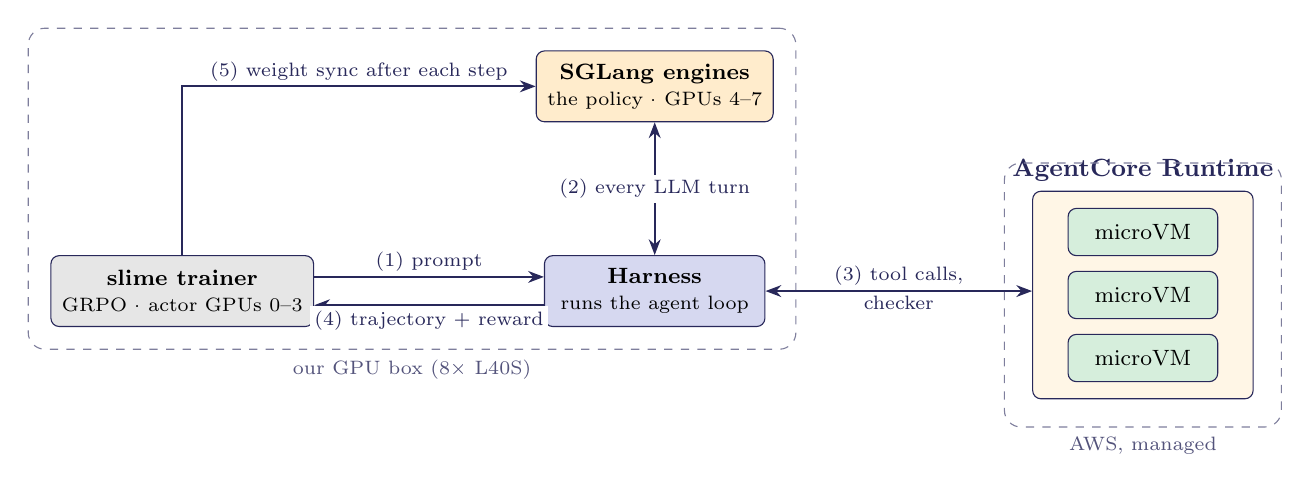
\begin{tikzpicture}[
  font=\footnotesize,
  box/.style={draw=ink, rounded corners=3pt, fill=#1, align=center, inner sep=4pt, minimum height=0.9cm, minimum width=2.8cm},
  line/.style={thick, draw=ink, -{Stealth[length=2mm]}},
  dline/.style={thick, draw=ink, {Stealth[length=2mm]}-{Stealth[length=2mm]}},
  head/.style={font=\small\bfseries, text=ink, align=center},
  lab/.style={font=\scriptsize, text=ink, fill=white, inner sep=1.5pt, align=center},
  note/.style={font=\scriptsize, text=ink!80, align=center},
  region/.style={draw=ink!60, dashed, rounded corners=6pt, inner sep=8pt},
]

\node[box=slime] (sl) at (0,0) {\textbf{slime trainer}\\\scriptsize GRPO · actor GPUs 0--3};
\node[box=host]  (h)  at (6,0) {\textbf{Harness}\\\scriptsize runs the agent loop};
\node[box=gpu]   (e)  at (6,2.6) {\textbf{SGLang engines}\\\scriptsize the policy · GPUs 4--7};
\node[box=vm, minimum width=1.9cm, minimum height=0.6cm] (v1) at (12.2,0.75) {microVM};
\node[box=vm, minimum width=1.9cm, minimum height=0.6cm] (v2) at (12.2,-0.05) {microVM};
\node[box=vm, minimum width=1.9cm, minimum height=0.6cm] (v3) at (12.2,-0.85) {microVM};
\begin{scope}[on background layer]
  \node[box=ac, fit=(v1)(v3), inner sep=6pt, label={[head]above:AgentCore Runtime}] (ac) {};
  \node[region, fit=(sl)(h)(e), label={[note]below:our GPU box (8× L40S)}] {};
  \node[region, fit=(ac), inner sep=10pt, label={[note]below:AWS, managed}] {};
\end{scope}
\draw[line] ($(sl.east)+(0,0.18)$) -- node[lab, above] {(1) prompt} ($(h.west)+(0,0.18)$);
\draw[line] ($(h.west)+(0,-0.18)$) -- node[lab, below] {(4) trajectory + reward} ($(sl.west-|sl.east)+(0,-0.18)$);
\draw[dline] (h) -- node[lab] {(2) every LLM turn} (e);
\draw[dline] (h.east) -- node[lab, above] {(3) tool calls,} node[lab, below] {checker} (ac.west|-h.east);
\draw[line] (sl.north) |- node[lab, pos=0.75, above] {(5) weight sync after each step} (e.west);
\end{tikzpicture}
\end{document}
